%%%%%%%%%%%%%%%%%%%%%%%%%%%%%%%%%%%%%%%%%
% Jacobs Landscape Poster
% LaTeX Template
% Version 1.0 (29/03/13)
%
% Created by:
% Computational Physics and Biophysics Group, Jacobs University
% https://teamwork.jacobs-university.de:8443/confluence/display/CoPandBiG/LaTeX+Poster
% 
% Further modified by:
% Nathaniel Johnston (nathaniel@njohnston.ca)
%
% This template has been downloaded from:
% http://www.LaTeXTemplates.com
%
% 
% Masaryk University presentation themes were downloaded from:
% https://www.overleaf.com/gallery/tagged/muni
%
% and ported into Jacobs Landscape Poster by:
% Jumaidil Awal (ideal1st.here@googlemail.com)
% 
% Jacobs Landscape Poster License:
% CC BY-NC-SA 3.0 (http://creativecommons.org/licenses/by-nc-sa/3.0/)
%
% Masaryk University's fibeamer theme license:
% Copyright 2015  Vít Novotný <witiko@mail.muni.cz>
% Faculty of Informatics, Masaryk University (Brno, Czech Republic)
% under Latex Project Public License
%
%%%%%%%%%%%%%%%%%%%%%%%%%%%%%%%%%%%%%%%%%

%----------------------------------------------------------------------------------------
%	PACKAGES AND OTHER DOCUMENT CONFIGURATIONS
%----------------------------------------------------------------------------------------

\documentclass[final]{beamer}

\usepackage[scale=1.24]{beamerposter} % Use the beamerposter package for laying out the poster

%\usetheme{confposter} % Use the confposter theme supplied with this template
\usetheme[faculty=chemo]{fibeamer} % Uncomment to use Masaryk University's fibeamer theme instead.

%\setbeamercolor{block title}{fg=ngreen,bg=white} % Colors of the block titles
%\setbeamercolor{block body}{fg=black,bg=white} % Colors of the body of blocks
%\setbeamercolor{block alerted title}{fg=white,bg=dblue!70} % Colors of the highlighted block titles
%\setbeamercolor{block alerted body}{fg=black,bg=dblue!10} % Colors of the body of highlighted blocks
% Many more colors are available for use in beamerthemeconfposter.sty

%-----------------------------------------------------------
% Define the column widths and overall poster size
% To set effective sepwid, onecolwid and twocolwid values, first choose how many columns you want and how much separation you want between columns
% In this template, the separation width chosen is 0.024 of the paper width and a 4-column layout
% onecolwid should therefore be (1-(# of columns+1)*sepwid)/# of columns e.g. (1-(4+1)*0.024)/4 = 0.22
% Set twocolwid to be (2*onecolwid)+sepwid = 0.464
% Set threecolwid to be (3*onecolwid)+2*sepwid = 0.708

\newlength{\sepwid}
\newlength{\onecolwid}
\newlength{\twocolwid}
\newlength{\threecolwid}
\setlength{\paperwidth}{46.8in} % A0 width: 46.8in
\setlength{\paperheight}{33.1in} % A0 height: 33.1in
\setlength{\sepwid}{0.024\paperwidth} % Separation width (white space) between columns
\setlength{\onecolwid}{0.21\paperwidth} % Width of one column
\setlength{\twocolwid}{0.451\paperwidth} % Width of two columns
\setlength{\threecolwid}{0.678\paperwidth} % Width of three columns
%\setlength{\topmargin}{-0.5in} % Reduce the top margin size
%-----------------------------------------------------------

\usepackage{graphicx}  % Required for including images

\usepackage{booktabs} % Top and bottom rules for tables

\usepackage{multicol} % For multicols

\usepackage{mdframed} % for border around figures

\usepackage{mathabx} % for up and down arrow

\usepackage{listings} % for C code
%----------------------------------------------------------------------------------------
%	TITLE SECTION 
%----------------------------------------------------------------------------------------

\title{A Preliminary Performance Model for Optimizing Software Packet Processing Pipelines} % Poster title
\author{Ankit Bhardwaj, Atul Shree, Bhargav Reddy V, and Sorav Bansal} % Author(s)
\institute{Department of Computer Science and Engineering, Indian Institute of Technology Delhi} % Institution(s)

%----------------------------------------------------------------------------------------

\begin{document}
\addtobeamertemplate{block end}{}{\vspace*{2ex}} % White space under blocks
\addtobeamertemplate{block example end}{}{\vspace*{2ex}} % White space under example blocks
\addtobeamertemplate{block alerted end}{}{\vspace*{2ex}} % White space under highlighted (alert) blocks

\setlength{\belowcaptionskip}{2ex} % White space under figures
\setlength\belowdisplayshortskip{2ex} % White space under equations
%\begin{darkframes} % Uncomment for dark theme, don't forget to \end{darkframes}
\begin{frame} % The whole poster is enclosed in one beamer frame

%==========================Begin Head===============================
  \begin{columns}
   \begin{column}{\linewidth}
    \vskip1cm
    \centering
    \usebeamercolor{title in headline}{\color{fg}\Huge{\textbf{\inserttitle}}\\[0.5ex]}
    \usebeamercolor{author in headline}{\color{fg}\Large{\insertauthor}\\[1ex]}
    \usebeamercolor{institute in headline}{\color{fg}\large{\insertinstitute}\\[1ex]}
    \vskip1cm
   \end{column}
   \vspace{1cm}
  \end{columns}
 \vspace{1cm}

%==========================End Head===============================

\begin{columns}[t] % The whole poster consists of three major columns, the second of which is split into two columns twice - the [t] option aligns each column's content to the top

\begin{column}{\sepwid}\end{column} % Empty spacer column

\begin{column}{\onecolwid} % The first column

%----------------------------------------------------------------------------------------
%	OBJECTIVES
%----------------------------------------------------------------------------------------

\begin{exampleblock}{Motivation and Objectives}
\textbf{Motivation}: With increasing popularity of SDN, newer protocols are being developed over time. Researcher are developing DSLs to make the task easier. However, ease of programming doesn't guarantee application performance.\\
\textbf{Goal}: Develop a compiler that can automatically map a high-level specification to an underlying machine architecture in an optimal way.
\end{exampleblock}

%----------------------------------------------------------------------------------------
%	Compilation
%----------------------------------------------------------------------------------------

\begin{exampleblock}{Compilation Phases}


\begin{figure}
\fbox{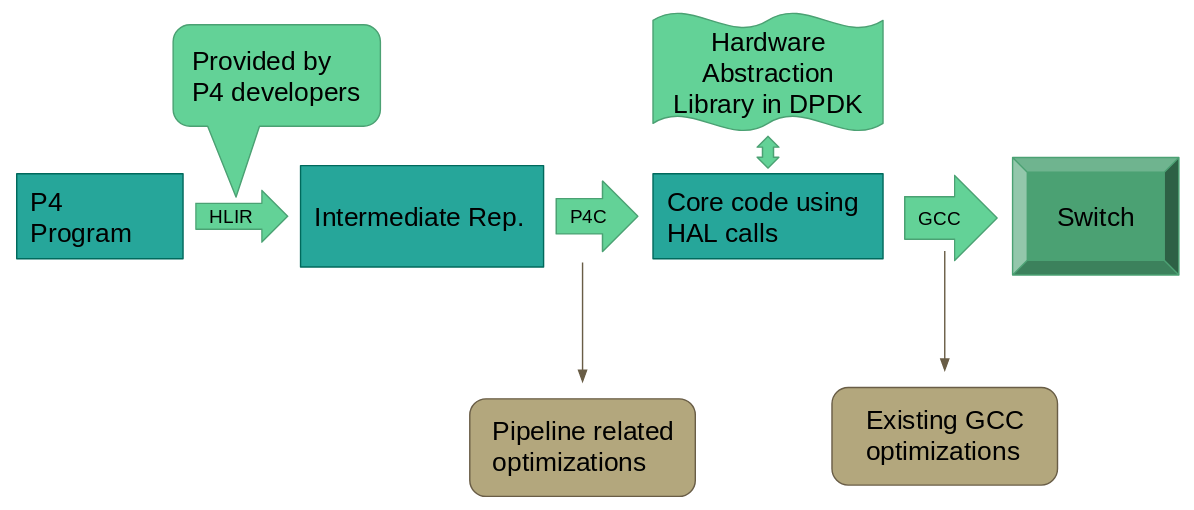
\includegraphics[width=0.8\linewidth]{img/compilation_phases}}
\caption{Compilation phases}
\end{figure}
Applications written in P4\cite{p4} are given as the input to P4C compiler and the compiler generated DPDK\cite{DPDK} based Applications. DPDK application is compiled using gcc to generate the target binary.
\end{exampleblock}

%----------------------------------------------------------------------------------------
%	Piplining
%----------------------------------------------------------------------------------------

\begin{exampleblock}{Packet Processing Pipeline}
\begin{figure}
\fbox{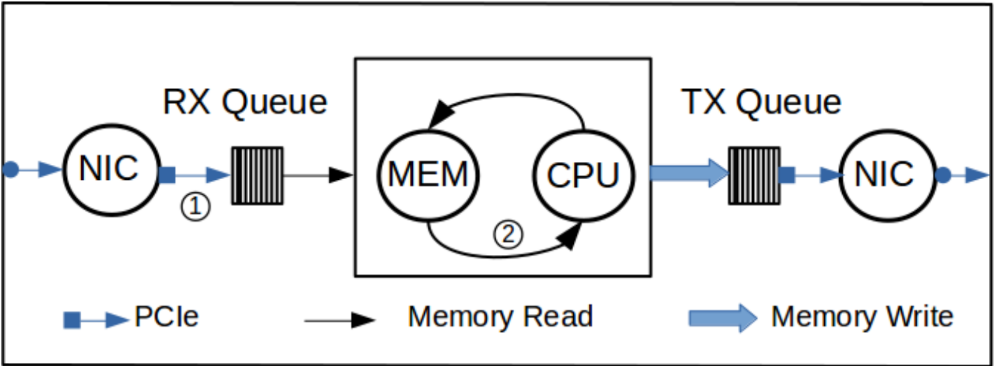
\includegraphics[width=0.8\linewidth]{img/packet_process_pipeline}}
\caption{Packet Processing Pipeline}
\end{figure}
\begin{enumerate}[*]
 \item Exploit DMA bandwidth between NIC and Main Memory labeled \textcircled{1} in Figure
 \item Exploit Memory Level Parallelism between CPU and Memory labeled \textcircled{2} in Figure
\end{enumerate}
\end{exampleblock}


%------------------------------------------------

%----------------------------------------------------------------------------------------

\end{column} % End of the first column

\begin{column}{\sepwid}\end{column} % Empty spacer column

\begin{column}{\twocolwid} % Begin a column which is two columns wide (column 2)

%\begin{columns}[t,totalwidth=\twocolwid] % Split up the two columns wide column



%\begin{column}{\twocolwid}
\begin{exampleblock}{Loop-Fission for Batching, Sub-Batching, and Prefetching}
\begin{multicols}{3}
%----------------------------------------------
%	BATCHING
%----------------------------------------------
\begin{figure}[ht]
\begin{tiny}
\begin{tabular}[b]{p{\onecolwid}}
sub app \{ \\
\hspace{0.2\sepwid}for (i = 0; i < B; i++) \{ \\
\hspace{0.4\sepwid}p = read\_from\_input\_NIC(); \\
\hspace{0.4\sepwid}p = process\_packet(p); \\
\hspace{0.4\sepwid}write\_to\_output\_NIC(p); \\
\hspace{0.2\sepwid}\}\\
\hspace{1\sepwid}$\updownarrows$\\
sub app \{\\
\hspace{0.2\sepwid}for (i = 0; i < B; i++)\\
\hspace{0.4\sepwid}p[i] = read\_from\_input\_NIC();\\
\hspace{0.2\sepwid}for (i = 0; i < B; i++)\\
\hspace{0.4\sepwid}p[i] = process\_packet(p[i]);\\
\hspace{0.2\sepwid}for (i = 0; i < B; i++)\\
\hspace{0.4\sepwid}write\_to\_output\_NIC(p[i]);\\
\}
\end{tabular}
\end{tiny}
% \caption{Batching}
\end{figure}
%----------------------------------------------
%	SUB-BATCHING
%----------------------------------------------
\begin{figure}[ht]
\begin{tiny}
\begin{tabular}[b]{p{\onecolwid}}
sub{ process\_packet}(p) \{ \\
\hspace{0.2\sepwid}for (i = 0; i < B; i++) \{ \\
\hspace{0.4\sepwid}t1 = lookup\_table1(p[i]); \\
\hspace{0.4\sepwid}t2 = lookup\_table2(p[i], t1); \\
\hspace{0.4\sepwid}\ldots\\
\hspace{0.2\sepwid}\}\hspace{0.2\sepwid}\}\\
\hspace{1\sepwid}$\updownarrows$\\
sub {process\_packet}(p) \{\\
\hspace{0.2\sepwid}for (i = 0; i < B; i+=b) \{\\
\hspace{0.4\sepwid}for (j = i; j < i+b; j++)\\
\hspace{0.6\sepwid}t1[j-i] = lookup\_table1(p[j]);\\
\hspace{0.4\sepwid}for (j = i; j < i+b; j++)\\
\hspace{0.6\sepwid}t1[j-i] = lookup\_table2(p[j], t1[j-i]);\\
\hspace{0.4\sepwid}\ldots\\
\hspace{0.2\sepwid}\}\hspace{0.2\sepwid}\}
\end{tabular}
\end{tiny}
% \caption{Sub-batching}
\end{figure}
%----------------------------------------------
%	PREFETCHING
%----------------------------------------------
\begin{figure}[ht]
\begin{tiny}
\begin{tabular}[b]{p{\onecolwid}}

sub\hspace{0.2\sepwid} hash\_lookup() \{\\
\hspace{0.4\sepwid}for( i=0; i<B; i++)\{\\
\hspace{0.6\sepwid}key\_hash[i] = hash\_compute(key[i]);\\
\hspace{0.6\sepwid}prefetch(bucket(key-hash[i]));\\
\hspace{0.4\sepwid}\}\\
\hspace{0.4\sepwid}for( i=0; i < B; i++)\{\\
\hspace{0.6\sepwid}val[j] = hash\_lookup(key\_hash[j]);\\
\}\hspace{0.4\sepwid}\}

\hspace{1\sepwid}$\updownarrows$\\
 
sub{ hash\_lookup()} \{\\
\hspace{0.4\sepwid}for( i = 0; i < B; i += b)\{\\
\hspace{0.6\sepwid}for( j = i; j < i + b; j++ )\{\\
\hspace{0.8\sepwid}key\_hash[i] = hash\_compute(key[i]);\\
\hspace{0.8\sepwid}prefetch(bucket(key-hash[i]));\\
\hspace{0.6\sepwid}\}\\
\hspace{0.6\sepwid}for( j = i; j < i + b; j++ )\{\\
\hspace{0.8\sepwid}val[j] = hash\_lookup(key\_hash[j]);\\
\}\hspace{0.4\sepwid}\}\hspace{0.2\sepwid}\}
\end{tabular}
\end{tiny}
% \caption{Prefetching}
\end{figure}

\end{multicols}
\end{exampleblock}
%----------------------------------------------------------------------------------------
%	IMPORTANT RESULT
%----------------------------------------------------------------------------------------

\begin{alertblock}{Performance Model}
% \begin{multicols}{2}
IO Subsystem, Memory Subsystem and CPU work in a pipeline fashion. Let the service rate of CPU, CPU-Memory, I/O-Memory DMA interface be c, m, d. $Throughput$ of the application will be $min(c, m, d)$. The value of b will vary with change in the parameters related to memory $f_{mem}(m, b)$. DMA interface is not linearly scalable and rate increases based on some function $f_{dma} (d,B)$.
$$Throughput = min(c, f_{mem}(m, b), f_{dma})(d, B))$$
\end{alertblock} 

%----------------------------------------------------------------------------------------

\begin{columns}[t,totalwidth=\twocolwid] % Split up the two columns wide column again
\begin{column}{\twocolwid} % The first column within column 2 (column 2.1)
\begin{exampleblock}{Experiments and Results}
\begin{multicols}{3}

\begin{figure}
\fbox{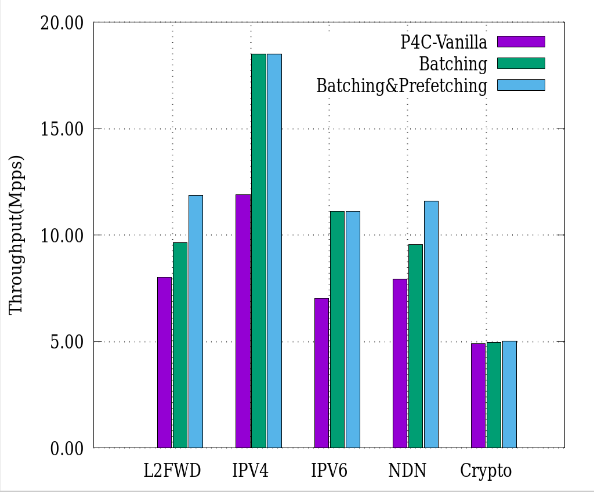
\includegraphics[width=0.99\linewidth]{img/batching_and_prefetching}}
\caption{Effect of Batching and Prefetching}
\end{figure}

\begin{figure}
\fbox{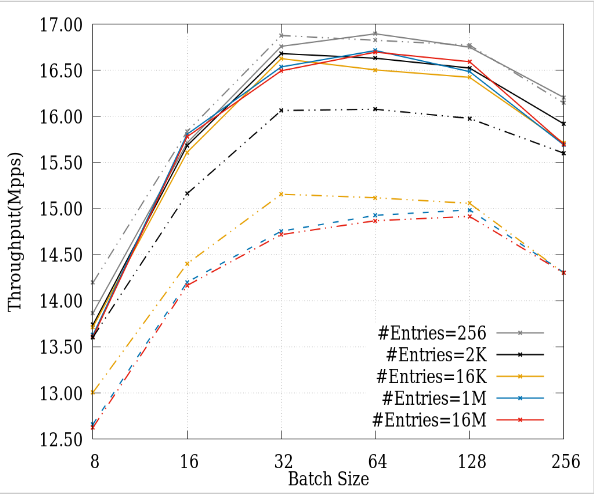
\includegraphics[width=0.99\linewidth]{img/throughput_sensitivity_B}}
\caption{Sensitivity of Throughput to B. Solid line b = B and dotted lines b = 1.}
\end{figure}

\begin{figure}
\fbox{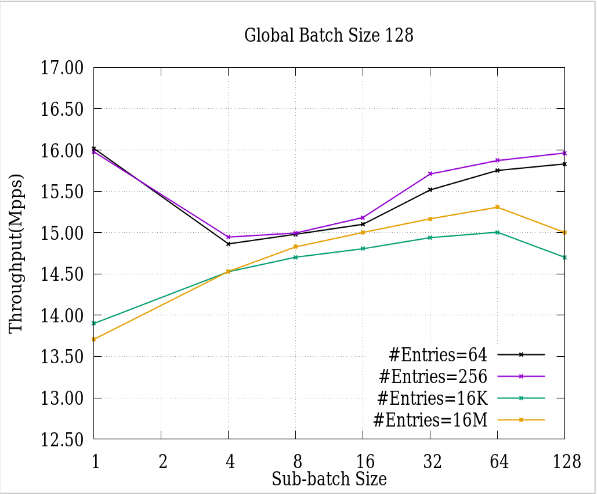
\includegraphics[width=0.99\linewidth]{img/throughput_sensitivity_b}}
\caption{Sensitivity of Throughput to b. Batch Size B = 128 for these experiments.}
\end{figure}

\end{multicols}
\end{exampleblock}

%----------------------------------------------------------------------------------------

\end{column} % End of column 2.1
\begin{column}{\sepwid}\end{column} % Empty spacer column

% 
% \begin{column}{\onecolwid} % The second column within column 2 (column 2.2)
% 
% %----------------------------------------------------------------------------------------
% %	RESULTS
% %----------------------------------------------------------------------------------------
% 
% \begin{exampleblock}{Results}
% 
% \begin{figure}
% 
\includegraphics[width=0.8\linewidth]{img/placeholder.jpg}
% \caption{Figure caption}
% \end{figure}
% 
% Nunc tempus venenatis facilisis. Curabitur suscipit consequat eros non porttitor. Sed a massa dolor, id ornare enim:
% 
% \begin{table}
% \vspace{2ex}
% \begin{tabular}{l l l}
% \toprule
% \textbf{Treatments} & \textbf{Response 1} & \textbf{Response 2}\\
% \midrule
% Treatment 1 & 0.0003262 & 0.562 \\
% Treatment 2 & 0.0015681 & 0.910 \\
% Treatment 3 & 0.0009271 & 0.296 \\
% \bottomrule
% \end{tabular}
% \caption{Table caption}
% \end{table}
% 
% \end{exampleblock}
% 
% %----------------------------------------------------------------------------------------
% 
% \end{column} % End of column 2.2

\end{columns} % End of the split of column 2

\end{column} % End of the second column

\begin{column}{\sepwid}\end{column} % Empty spacer column

% ---------------------------------------------------------------------------------------
% Column 3
% ---------------------------------------------------------------------------------------

\begin{column}{\onecolwid} % The third column

%----------------------------------------------------------------------------------------
%	CONCLUSION
%----------------------------------------------------------------------------------------

\begin{exampleblock}{Conclusion}
We are using Batching(B) to exploit available parallelism between NIC and Memory interface, and prefetching to exploit the memory level parallelism between CPU and Memory interface.
Sub-Batching(b) is being used to adjust the prefetch distance to take full advantage from software prefetching. The model to get the optimal value of b and B is preliminary and not fully automatic. We are running the applications to get the value of b and B and feeding the compiler to generate the optimal code. These optimizations can be used for wide variety of network and streaming applications.
\end{exampleblock}

%----------------------------------------------------------------------------------------
%	ADDITIONAL INFORMATION
%----------------------------------------------------------------------------------------

\begin{exampleblock}{Future Work}
\begin{itemize}
\item Get more understanding of NIC-Memory interface and CPU-Memory interface. 
\item Make the model robust to be used for various kind of applications.
\item Use the model for various architecture and do the appropriate changes.
\end{itemize}
\end{exampleblock}

%----------------------------------------------------------------------------------------
%	REFERENCES
%----------------------------------------------------------------------------------------

\begin{exampleblock}{References}

\nocite{*} % Insert publications even if they are not cited in the poster
\small{\bibliographystyle{unsrt}
\bibliography{sample}\vspace{1cm}}
\end{exampleblock}

%----------------------------------------------------------------------------------------
%	ACKNOWLEDGEMENTS
%----------------------------------------------------------------------------------------

%\setbeamercolor{block title}{fg=red,bg=white} % Change the block title color

%\begin{exampleblock}{Acknowledgements}

%\small{\rmfamily{Nam mollis tristique neque eu luctus. Suspendisse rutrum congue nisi sed convallis. Aenean id neque dolor. Pellentesque habitant morbi tristique senectus et netus et malesuada fames ac turpis egestas.}} \\

%\end{exampleblock}

%----------------------------------------------------------------------------------------
%	CONTACT INFORMATION
%----------------------------------------------------------------------------------------

%\setbeamercolor{block alerted title}{fg=black,bg=norange} % Change the alert block title colors
%\setbeamercolor{block alerted body}{fg=black,bg=white} % Change the alert block body colors

% \begin{block}{Contact Information}
% \begin{itemize}
% \item Web: \href{http://ideal1st.com/}{http://ideal1st.com/}
% \item Email: \href{mailto:ideal1st.here@gmail.com}{ideal1st.here@gmail.com}
% \end{itemize}
% \end{block}

\begin{center}

\includegraphics[width=0.7\linewidth]{img/iitd_logo.jpg}
\end{center}




%----------------------------------------------------------------------------------------

\end{column} % End of the third column

\begin{column}{\sepwid}\end{column} % Empty spacer column

\end{columns} % End of all the columns in the poster

\end{frame} % End of the enclosing frame
%\end{darkframes} % Uncomment for dark theme
\end{document}
